\section{\ce{[Co(SCN)_2(4-methoxypyridine)_4]}}
\subsection{Synthesis}
0.58 g \ce{Co(NO_3)_2* 6 H_2O} (2 mmol), 0.38 g KSCN (4 mmol) and 0.87 g 4-methoxy-pyridine (8 mmol) were dissolved in 40 mL distilled \ce{H_2O}. The solution was heated up to $70^\circ$C  and stirred for 1 hour. After filtration the clear pink solution was placed in the drying oven ($70^\circ$C) overnight and then cooled down to RT. After a few hours pink crystals were obtained.
Anal. Calculated for \ce{C_{26}H_{28}CoN_{6}O_{4}S_{2}} (611,59 g/mol): 51.06\% C; 4.61\% H; 13.74\% N; 10.49 \% S;
Found: 50.94 \% C; 4.65\% H; 13.80 \% N; 10.30\% S;
IR (ATR, cm$^{-1}$): 2061 (s), 1608 (s), 1567 (s), 1508 (s), 1493 (s), 1460 (w), 1426 (m), 1293 (s), 1205 (s), 1024 (vs), 822 (s), 659 (w), 540 (s), 458 (m)

\begin{figure}[h!]
\centering
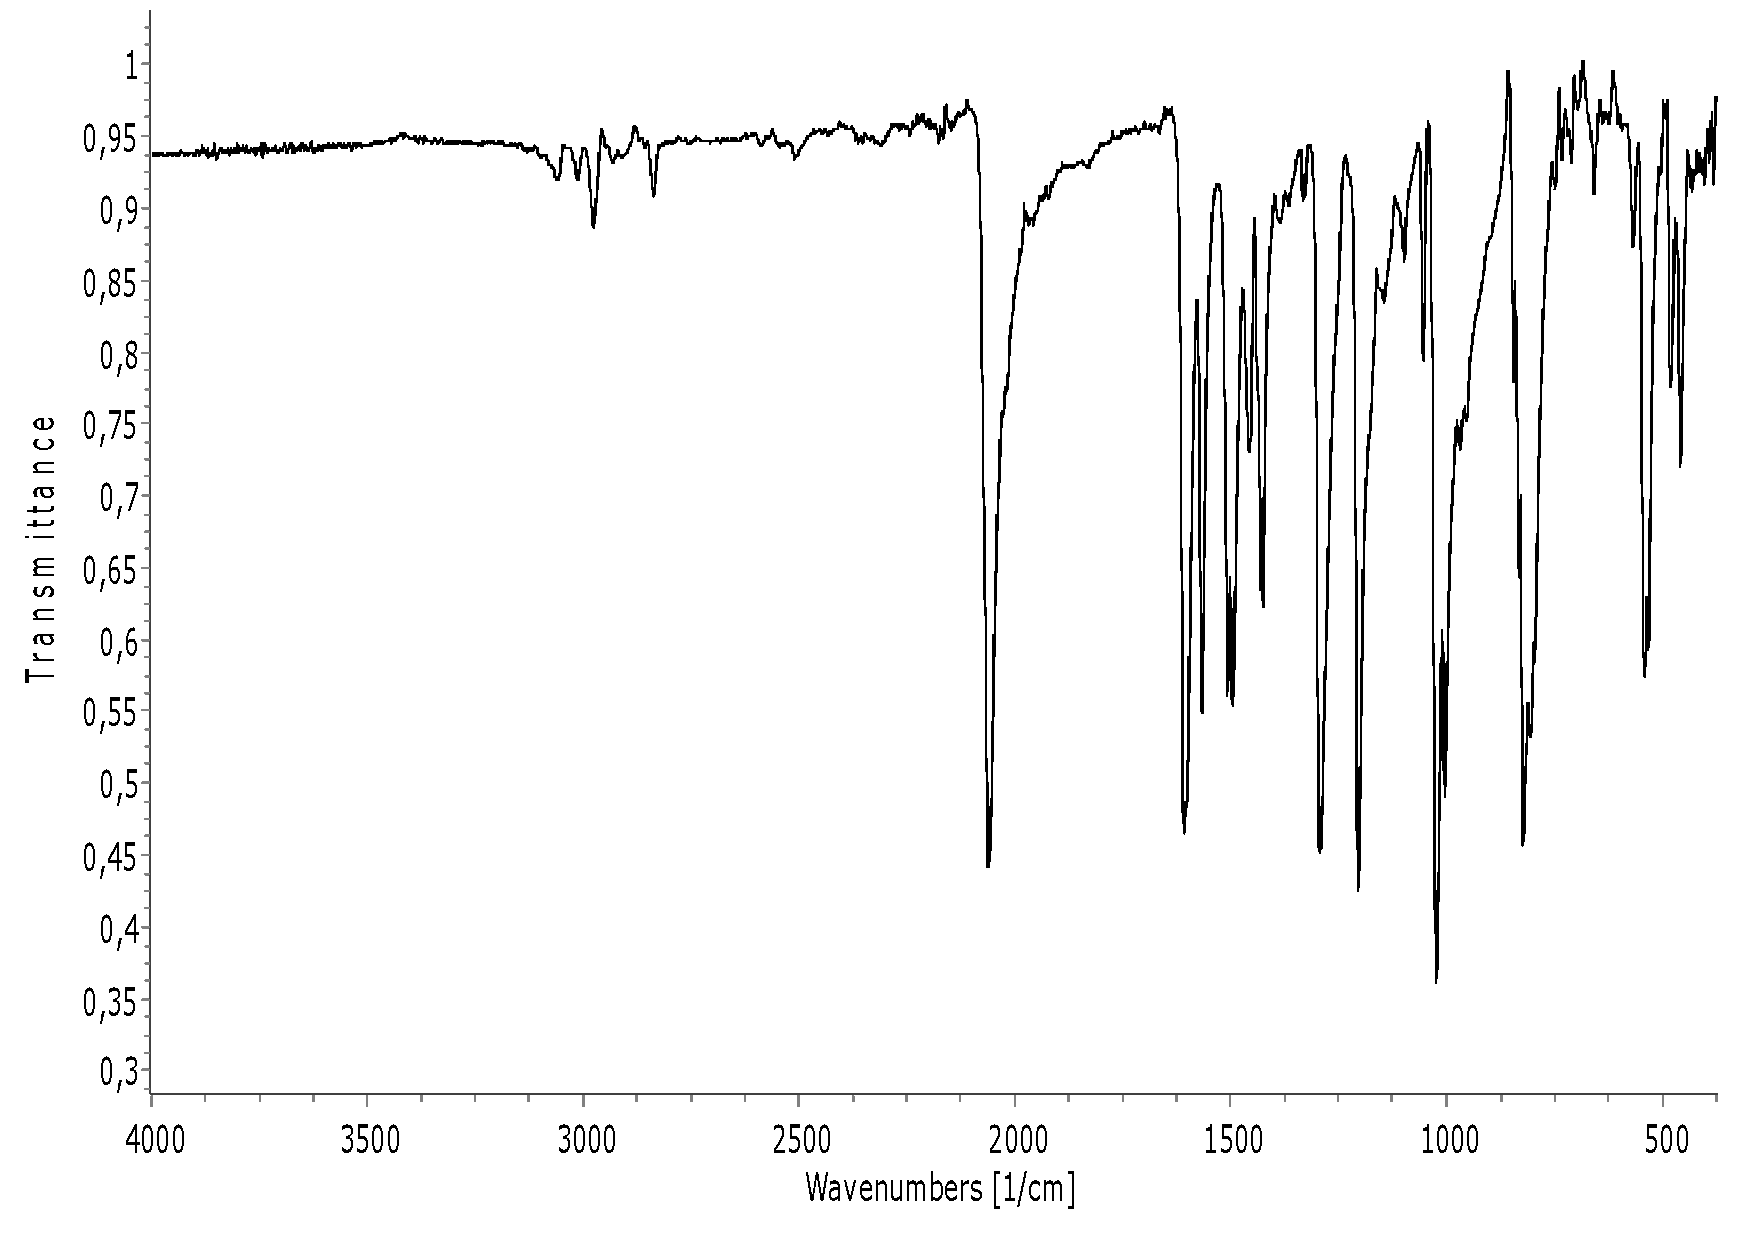
\includegraphics[width=1\textwidth]{figures/CoR4MOP-IR.pdf}
\caption{IR spectrum of \ce{[Co(SCN)_2(4-MeOpy)_4]}}
\end{figure}





\subsection{Structural characterization}

The crystal structure of \ce{[Co(SCN)_2(4-MeOpy)_4]}) consists of mononuclear and neutral Co(II) complexes. A perspective view is shown in fig. \ref{fig:CoR4MOP_pv}, a packing view in fig \ref{fig:CoR4MOP_packv} and selected bond parameters are summarized in table \ref{batlb:CoR4MOP}. Co(1) is six-coordinated by N atoms of two terminal isothiocyanato anions, further by N donor atoms of four neutral 4-methoxypyridine molecules. The \ce{CoN6} chromophore may be described as a slighly distorted octahedron with trans-arrangement of the isothiocyanato ligands. The Co-N bond lengths range from 2.089(5) to 2.195(5) \AA, and the transoid N-Co-N bond angles within the \ce{CoN6} octahedra vary from 175.08(17) to 178.96(18)$^\circ$. The bond parameters of the terminal isothiocyanato anions are: Co-N-C: 153.9(4) and 163.4(5)$^\circ$, N-C-S: 178.0(5) and 179.4(6)$^\circ$, N-C: 1.160(7) and 1.167(7) \AA, C-S: 1.637(5) and 1.628(6) \AA.The shortest metal-metal separation is 9.1969(19) \AA. 

\begin{table}[htpb!]
\centering
\captionabove{Selected bond lengths (\AA) and angles ($^\circ$) for \ce{[Co(SCN)_2(4-MeOpy)_4]}}
\begin{tabular}{|l|l|l|l|}
\hline
Co(1)-N(1) & 2.096(5) & Co(1)-N(4) & 2.195(5)\\
\hline
Co(1)-N(2) & 2.089(5) & Co(1)-N(5) & 2.136(5)\\
\hline
Co(1)-N(3) & 2.174(5) & Co(1)-N(6) & 2.155(5)\\
\hline
N(1)-C(1) & 1.160(7) & C(1)-S(1) & 1.637(5)\\
\hline
N(2)-C(2) & 1.167(7) & C(2)-S(2) & 1.628(6)\\
\hline
\hline
N(1)-Co(1)-N(2) & 178.96(18) & N(3)-Co(1)-N(5) & 175.08(17)\\
\hline
N(4)-Co(1)-N(6) & 1.178.44(17) & Co(1)-N(2)-C(2) & 153.9(4)\\
\hline
Co(1)-N(1)-C(1) & 163.4(5) & N(2)-C(2)-S(2) & 178.0(5)\\
\hline
N(1)-C(1)-S(1) & 179.4(6) & & \\
\hline
\end{tabular}
\label{batlb:CoR4MOP}
\end{table}



\begin{figure}[!htpb]
\centering
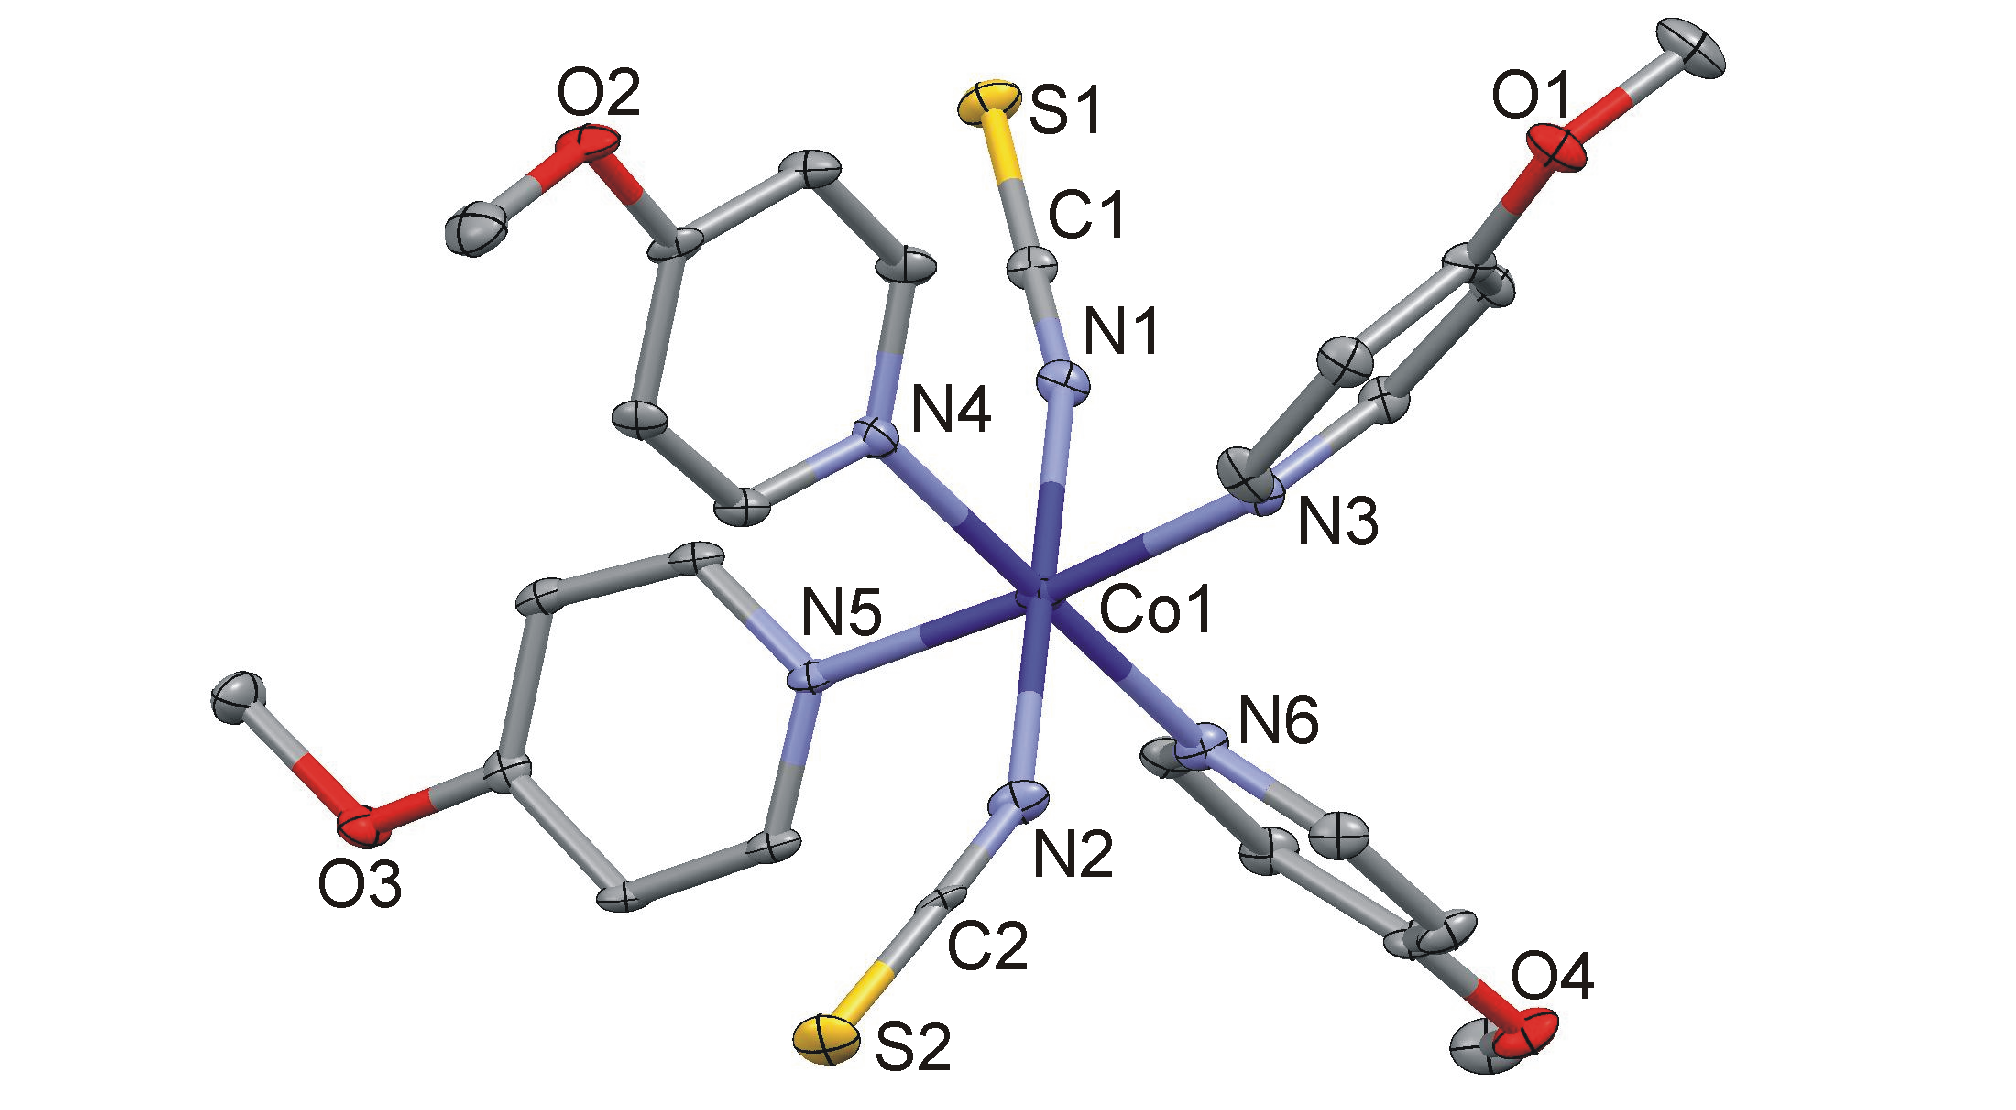
\includegraphics[width=1\textwidth]{figures/cormop_FIGm11.png}
\caption[Perspective view of \ce{[Co(SCN)_2(4-MeOpy)_4]}]{Perspective view of \ce{[Co(SCN)_2(4-MeOpy)_4]} with the atom numbering scheme.}
\label{fig:CoR4MOP_pv}
\vspace{\floatsep}
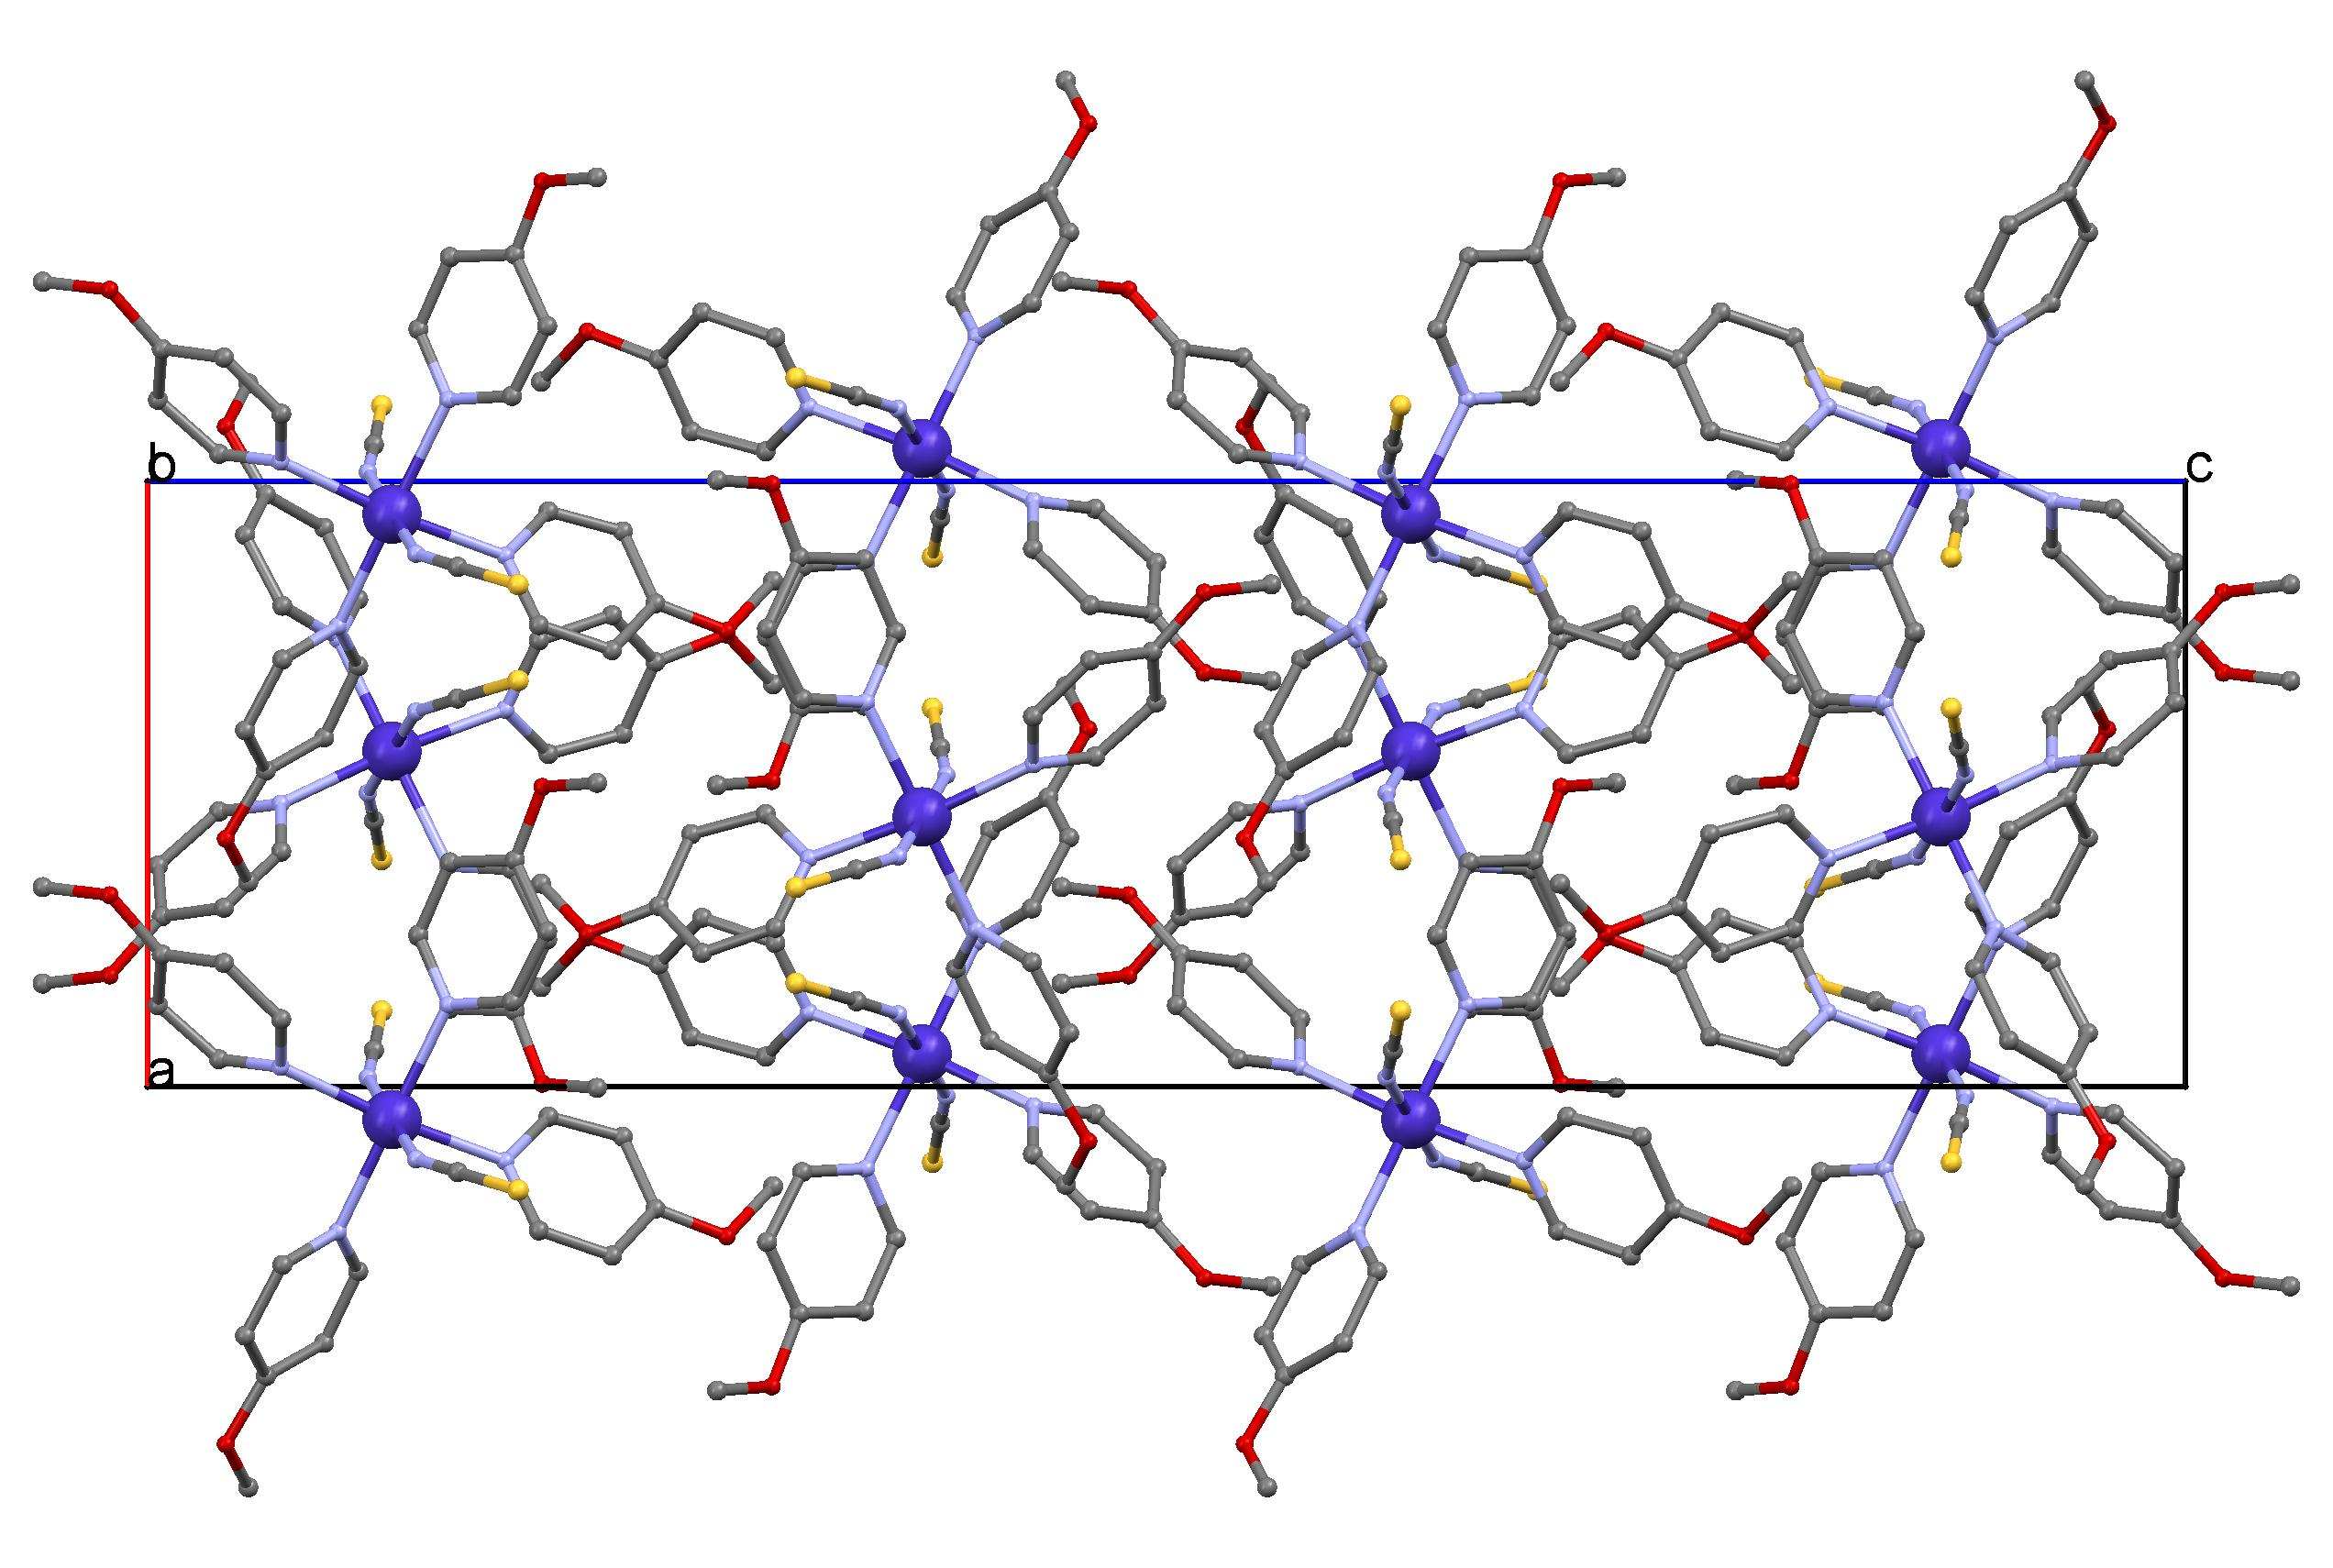
\includegraphics[width=1\textwidth]{figures/cormop_CB.png}
\caption{Packing view  of \ce{[Co(SCN)_2(4-MeOpy)_4]}.}
\label{fig:CoR4MOP_packv}
\end{figure}


\renewcommand{\arraystretch}{1.5}
\begin{table}
\centering
\captionabove{Crystallographic data and processing parameter of \ce{[Co(SCN)_2(4-MeOpy)_4]}}
\begin{tabular}{ | l |  l | }
\hline
Empirical formula & \ce{C_{26}H_{28}CoN_{6}O_{4}S_{2}}\\
\hline
Formula mass & 611.59\\
\hline
System & orthorhombic\\
\hline
Space group & Pbca\\
\hline
a ({\AA}) & 10.1815(17)\\
\hline
b ({\AA}) & 16.574(3)\\
\hline
c ({\AA}) & 34.268(6)\\
\hline
$\alpha$ ($^\circ$) & 90\\
\hline
$\beta$ ($^\circ$) & 90\\
\hline
$\gamma$ ($^\circ$) & 90\\
\hline
V (\AA$^{3}) $  & 5782.6(17)\\
\hline
Z & 8\\
\hline
T (K) & 100(2)\\
\hline
$\mu$ (mm$^{-1}$) & 0.780\\
\hline
 D$_{calc}$ (Mg/m$^{3}$) & 1.405\\
\hline
Crystal size (mm) & 0.19 x 0.16 x 0.09\\
\hline
$\theta$ max ($^\circ$) & 25.50\\
\hline
Data collected & 33321\\
\hline
Unique refl./ R$_{int}$ & 5372 / 0.1050\\
\hline
Parameters & 356\\
\hline
Goodness-of-Fit on F$^{2}$ & 1.154\\
\hline
R1 / wR2 (all data) & 0.0763 /0.1570\\
\hline
Residual extrema (e/\AA$^{3}$) & 0.64 /-0.85\\
\hline
\end{tabular}

\label{ptab:CoR4MOP}

\end{table}


